\documentclass[xcolor=svgnames]{beamer}
\usetheme[
    %%% options passed to the outer theme
    %    hidetitle,           % hide the (short) title in the sidebar
    %    hideauthor,          % hide the (short) author in the sidebar
    %    hideinstitute,       % hide the (short) institute in the bottom of the sidebar
    %    shownavsym,          % show the navigation symbols
         width=1.5cm,         % width of the sidebar (default is 2 cm)
    %    hideothersubsections,% hide all subsections but the subsections in the current section
    %    hideallsubsections,  % hide all subsections
         left                 % right of left position of sidebar (default is right)
    %%% options passed to the color theme
        lightheaderbg         % use a light header background
  ]{AAUsidebar}
\setbeameroption{show notes}

% #### graphics and schemes
\usepackage{graphicx}
\graphicspath{{img/}}
\usepackage{tikz}
\usetikzlibrary{                          % TikZ libraries
                scopes,                   % .
                shapes,                   % .
                arrows,                   % .
                through,                  % .
                calc,                     % .
                intersections,            % .
                spy,                      % .
                matrix,                   % .
                chains,                   % .
                mindmap,                  % .
                trees,                    % .
                decorations.pathreplacing,% .
                decorations.pathmorphing, % .
                decorations.markings}     % .

\usepackage{pgfplots}                     % TikZ plots
\usepackage{pgfplotstable}                % TikZ tables from CSV
\pgfplotsset{compat=1.3}                  % activates \xilabel shift` for pgfplots
\usepackage{array}
\usepackage{listings}
\usepackage{times}
\usepackage{amsmath}
\usepackage{verbatim}
\usepackage{ccicons}
\usepackage{tcolorbox}
\usepackage{chronosys}
\usepackage{listings}                     % code
\usepackage{adjustbox}                    % code
\usepackage{attrib}

% #### colors
\usepackage{xcolor}                       % common color names
\usepackage{colortbl}                     % common color names

% #### layouts
\usepackage{multicol}
\usepackage[textfont=footnotesize,bf]{caption}
\usepackage{subfig}

% #### fonts
\usepackage[utf8]{inputenc}
\usepackage[english]{babel}
\usepackage[T1]{fontenc}
\usepackage{cmbright}
\usepackage{soul} %slanted text
\usepackage{hyperref}
\urlstyle{same}
\hypersetup{pdfauthor={Francesco de Virgilio},pdftitle={New altmetrics for books: the HIRMEOS project}}

% #### tables
\usepackage{booktabs}			          % migliora la qualità delle tabelle
\usepackage{tabularx}			          % colonne a spaziatura fissa delle tabelle
\newcommand{\otoprule}                    % better top rule horizontal line
    {\midrule[\heavyrulewidth]}           % .


\begin{document}

\usebackgroundtemplate{
    
\includegraphics[width=\paperwidth,height=\paperheight]{img/cover}
}

    \begin{frame}[plain,noframenumbering]
        \begin{center}
            \color{RoyalBlue}
            \textbf{
                \Huge{New altmetrics for books}\\
                \Large{The HIRMEOS project}\\
            }
            \vspace{40pt}
            Francesco de Virgilio\\
            \vspace{8pt}
            \scriptsize{Tech Team Lead, Ubiquity Press}\\
            \scriptsize{Toronto, 27/09/2017}
        \end{center}
    \end{frame}

\usebackgroundtemplate{%
    
\includegraphics[width=\paperwidth,height=\paperheight]{img/background}
}

\section{The company}

    \subsection{Mission}

        \begin{frame}{What's Ubiquity Press?}
            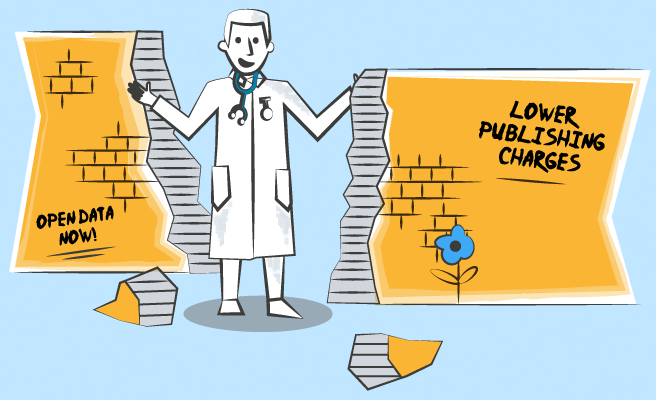
\includegraphics[width=0.7\textwidth]{img/up_banner}
            \begin{block}{Mission}
                To return control of publishing to universities, libraries, societies and researchers, providing them with the infrastructure and support to not only match but to outcompete the legacy publishers.
            \end{block}
        \end{frame}

    \subsection{Background}

        \begin{frame}{What's Ubiquity Press?}
            \begin{itemize}
                \item Spun out of University College London in 2012
                \item Researcher-led
                \item Grown out of the humanities
                \item 100+ years publishing experience
                \item Comprehensive approach: journals,
                \item books, data, software, wetware…
                \item Offices in London and Oakland
                \item Open access only
                \item we are interested in tech...
            \end{itemize}
        \end{frame}

\section{The project}

    \subsection{Definition}


        \begin{frame}{HIRMEOS}
            \begin{center}
                
\includegraphics[width=0.7\textwidth]{img/hirmeos}
                \color{black}
                \begin{block}{It's about monographies}
                    High Integration of Research Monographs in the European Open Science (Humanities and Social Sciences)
                \end{block}
            \end{center}
        \end{frame}

    \subsection{Open Access / Science}

        \begin{frame}{Open Access vs Open Science}
            Releasing millions of Open Access documents is \textbf{not enough}
            \pause
            we need to \textbf{interlink} them
            \pause
            via \textbf{useful} services
            \pause
            and build an \textbf{integrated trusted open knowledge system} across disciplines.
        \end{frame}

        \begin{frame}{Open Access vs Open Science}
            \vspace{0.05\textheight}
            \begin{columns}[c]
                \column{.5\textwidth}
                    Upstream
                    \begin{itemize}
                        \item<2-> opening the research process
                        \item<3-> access to methods, software, data and intermediary documents beyond the final peer-reviewed research article
                    \end{itemize}
                \column{.5\textwidth}
                    Downstream
                    \begin{itemize}
                        \item<4-> opening the knowledge discipline-based silos
                        \item<5-> creating bridges among countries and disciplines
                        \item<6-> supporting aggregation and reuse along interdisciplinary topics
                    \end{itemize}
            \end{columns}
        \end{frame}

    \subsection{Key concepts}

        \begin{frame}{Open Access vs Open Science}
            \vspace{0.05\textheight}
            \begin{columns}[c]
                \column{.3\textwidth}
                    Identification 
                    \begin{itemize}
                        \item<2-> author (OrcID)
                        \item<3-> document (DOI)
                        \item<4-> funding (Fundref)
                    \end{itemize}
                \column{.3\textwidth}
                    Recognition
                    \begin{itemize}
                        \item<5-> persons
                        \item<6-> dates
                        \item<7-> locations
                        \item<8-> indexed!
                    \end{itemize}
                \column{.3\textwidth}
                    Certification
                    \begin{itemize}
                        \item<9-> description of peer-review process
                        \item<10-> description of licence (DOAB)
                    \end{itemize}
            \end{columns}
        \end{frame}

        \begin{frame}{Open Access vs Open Science}
            \begin{columns}[c]
                \column{1\textwidth}
                    Advanced content
                    \begin{itemize}
                        \item<2-> open annotations (hypothesi.is)
                        \item<3-> usage metrics (downloads)
                        \item<4-> \textbf{altmetrics}
                    \end{itemize}
            \end{columns}
        \end{frame}

\section{Altmetrics}

    \usebackgroundtemplate{%
        
\includegraphics[width=\paperwidth,height=\paperheight]{img/white_back}
    }

        \begin{frame}{HIRMEOS Altmetrics}
            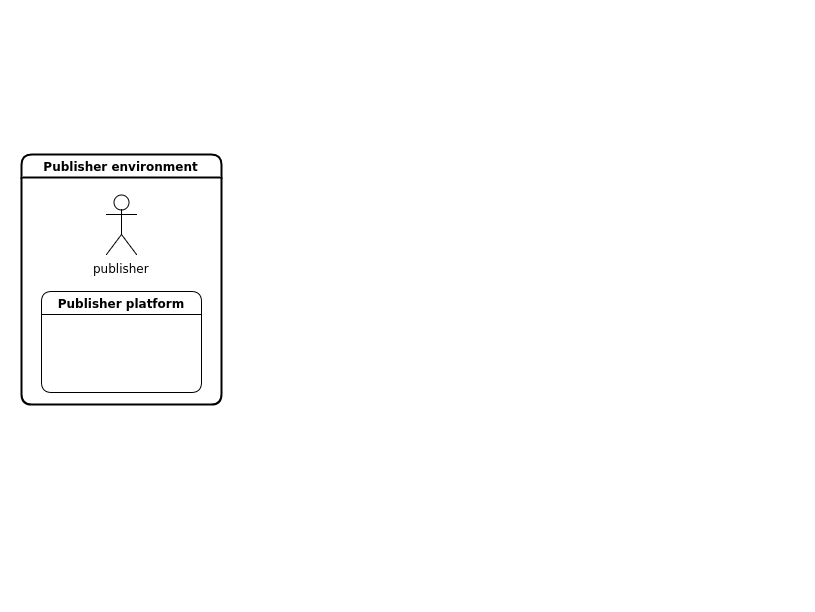
\includegraphics[width=0.9\textwidth]{img/h1}
        \end{frame}

        \begin{frame}{HIRMEOS Altmetrics}
            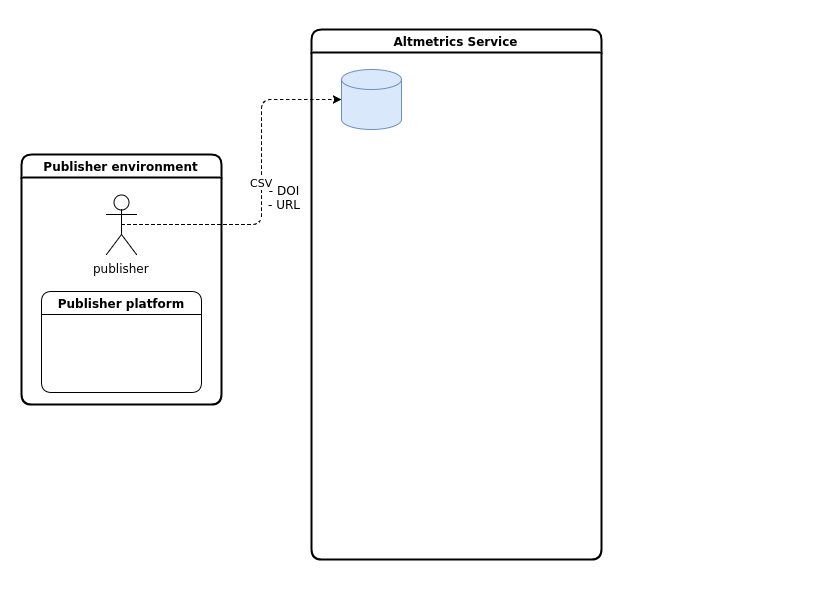
\includegraphics[width=0.9\textwidth]{img/h2}
        \end{frame}

        \begin{frame}{HIRMEOS Altmetrics}
            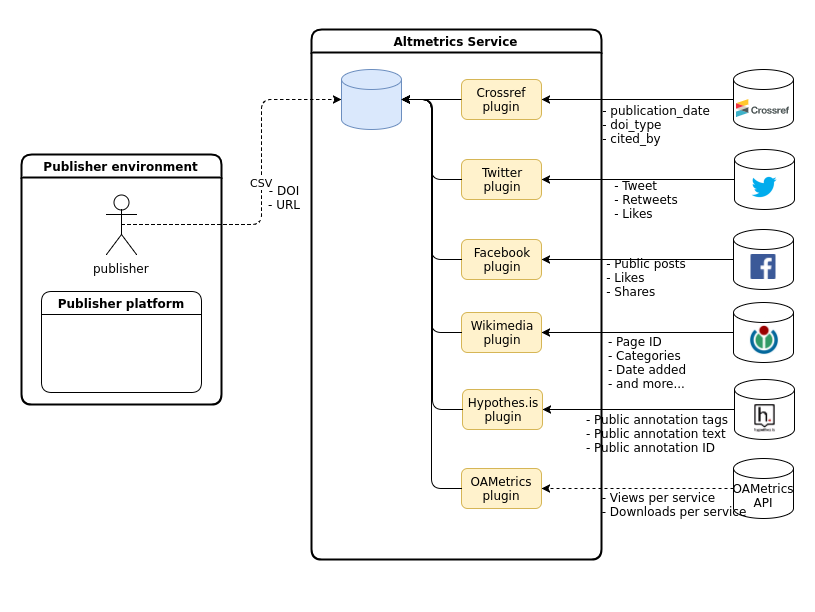
\includegraphics[width=0.9\textwidth]{img/h3}
        \end{frame}

        \begin{frame}{HIRMEOS Altmetrics}
            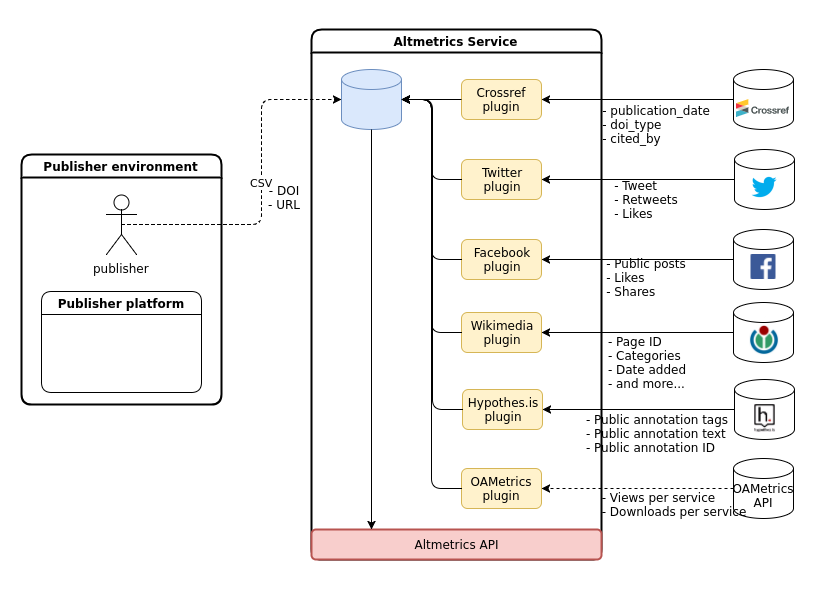
\includegraphics[width=0.9\textwidth]{img/h4}
        \end{frame}

        \begin{frame}{HIRMEOS Altmetrics}
            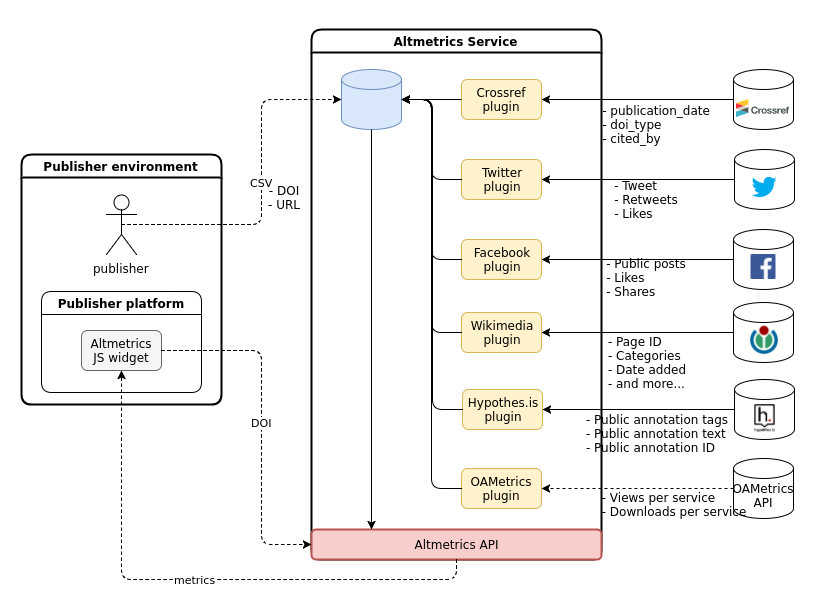
\includegraphics[width=0.9\textwidth]{img/h5}
        \end{frame}

\end{document}
